\documentclass{article}
\usepackage[margin=1in]{geometry}
\usepackage[utf8]{inputenc}
\usepackage{amsmath}
\usepackage{tikz}
\usepackage{pgfplots}
\pgfplotsset{compat=1.18}
\usepackage{color}
\usepackage{amsfonts}
\usepackage{amssymb}
\usepackage{graphicx}

\title{P.S. 6}
\author{Giacomo Cappelletto}
\date{\today}

\begin{document}

\maketitle

\section*{1}

\subsection*{A}

\subsubsection*{I}

\[
	det(A_1) = 0 \times 0 - 1 \times 1 = -1
\]

\subsubsection*{II}

\[
	det(A_2) = 2 \times 1 - 0 \times 0 = 2
\]

\subsubsection*{III}

\[
	det(A_3) = 1 \times 1 - 0 times -0.5 = 1
\]

\subsubsection*{IV}

\[
	det(A_4) = 1 \times 0 - 0 \times 0 = 0
\]

\subsubsection*{V}

\[
	det(A_5) = \frac{1}{2} \times \frac{1}{2} - (-\frac{\sqrt{3}}{2} \times \frac{\sqrt{3}}{2}) = \frac{1}{4} + \frac{3}{4} = 1
\]

\subsubsection*{VI}

\[
	det(A_6) = \cos{\theta} \times \cos{theta} - (-\sin{\theta} \times \sin{\theta}) = \cos^2{\theta} + \sin^2{\theta} = 1
\]

\subsection*{B}

One geometric representation of the determinant is the area of the parallelepiped (or parallelogram in this case in \(\mathbb{R}^2\)) which is spanned by the columns of the matrix \(A\). Since the entries have to be linearly in dependent for there to be an inverse. If the determinant is \(0\) then the vectors are in the same direction, not spanning any area, and therefore are linearly dependent. Therefore, the transofrmations which are invertible (those where \(|A_n| \neq 0\)) are \(\mathbf{I, II, III, V, VI}\).

\subsection*{C}

Since the determinant of a transformation gives the area scaling it will apply to any closed path, the size or area of \(C\) is equal to the size or area of \(B \times |A_n|\).

\subsection*{D}



\textbf{Contents}

\begin{itemize}
	\setlength{\itemsep}{-1ex}
	\item Load in the coordinates of vectors representing points on our "potato"
	\item EXAMPLE of applying a transformation to the potato's points
	\item YOUR ANSWERS
\end{itemize}
\begin{verbatim}
% Computational Linear Algebra (EK 103), Spring 2025, Boston University
% Problem Set 7, Problem 1(d), plotting transformations of a potato
% March 2025

% Set up the workspace
clear all; close all; clc;
\end{verbatim}


\textbf{Load in the coordinates of vectors representing points on our "potato"}

\begin{verbatim}
coord_filename = "potato_points.csv";
try
    pts = readmatrix(coord_filename);
catch anyerror
    disp("ERROR! Couldn't find potato_points.csv. Is it in the same directory as 
    ps7_problem1d.m ?? Check the homework instructions!");
    return
end
\end{verbatim}


\textbf{EXAMPLE of applying a transformation to the potato's points}

\begin{verbatim}
% the identity matrix should keep the potato where it is
I = [1, 0;
     0, 1];
pts_example = I*pts;

% This is just to check you've got the right files here, no need for more
% of the "try catch" stuff more than once.
try
    plot_potatoes(pts, pts_example, "Identity Matrix");
catch anyerr
    disp("Error! Couldn't find the function that plots our potato points.
    Is plot_potatoes.m in the same directory as ps7_problem1d.m ??")
    return
end
\end{verbatim}

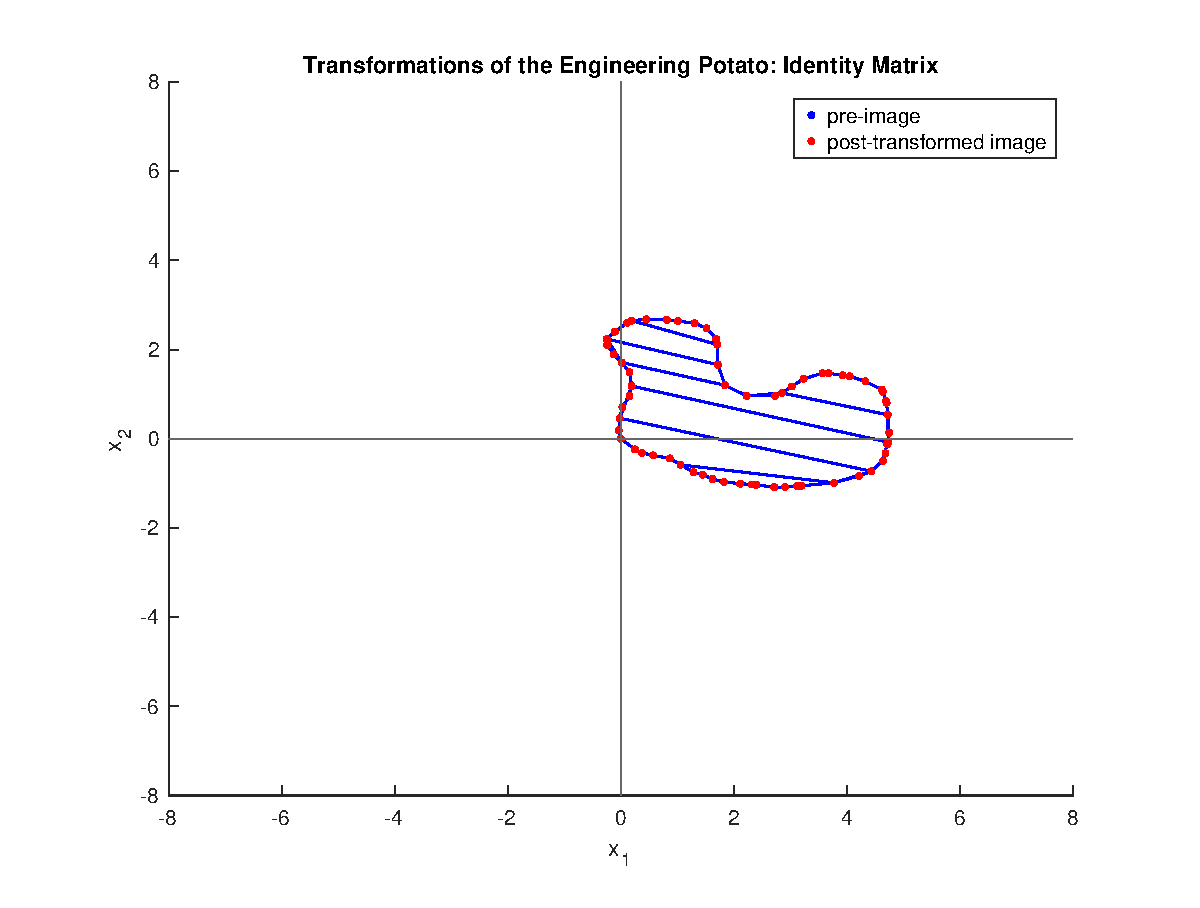
\includegraphics [width=4in]{1.eps}


\textbf{YOUR ANSWERS}

\begin{verbatim}
% 1(c) (i)
A1 = [0,1;1,0]
pts1 = A1*pts;
plot_potatoes(pts, pts1, "A1");

% 1(c) (ii)
A2 = [1,0;0,2]
pts2 = A2*pts;
plot_potatoes(pts, pts2, "A2");

% 1(c) (iii)
A3 = [1,0;-0.5,1]
pts3 = A3*pts;
plot_potatoes(pts, pts3, "A3");

% 1(c) (iv)
A4 = [1,0;0,0]
pts4 = A4*pts;
plot_potatoes(pts, pts4, "A4");

% 1(c) (v)
% Note for those new to matlab: sqrt(x) gives you the square root of x.
A5 = [0.5, (-sqrt(3))/2;(sqrt(3))/2, 0.5]
pts5 = A5*pts;
plot_potatoes(pts, pts5, "A5");
\end{verbatim}

\color{lightgray} \begin{verbatim}
A1 =

     0     1
     1     0


A2 =

     1     0
     0     2


A3 =

    1.0000         0
   -0.5000    1.0000


A4 =

     1     0
     0     0


A5 =

    0.5000   -0.8660
    0.8660    0.5000

\end{verbatim} \color{black}

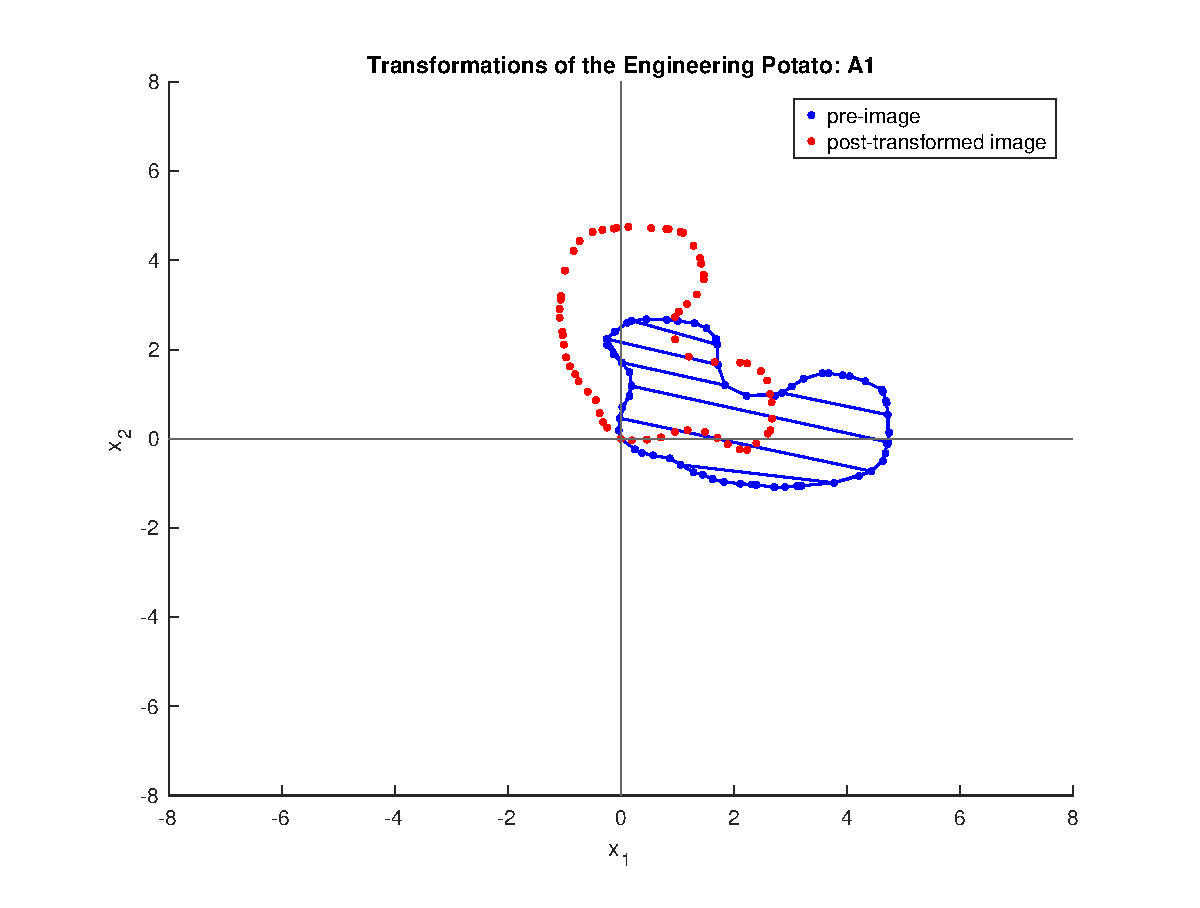
\includegraphics [width=4in]{2.eps}

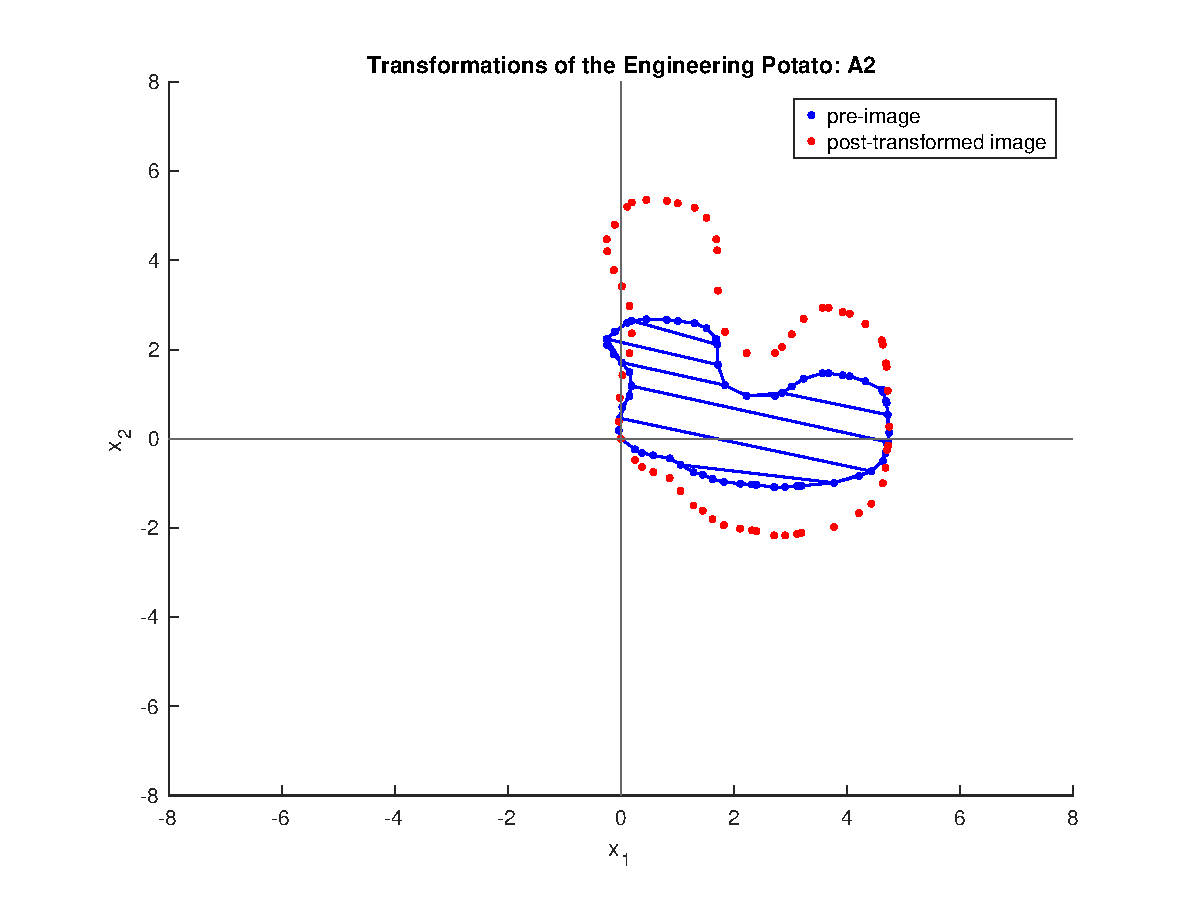
\includegraphics [width=4in]{3.eps}

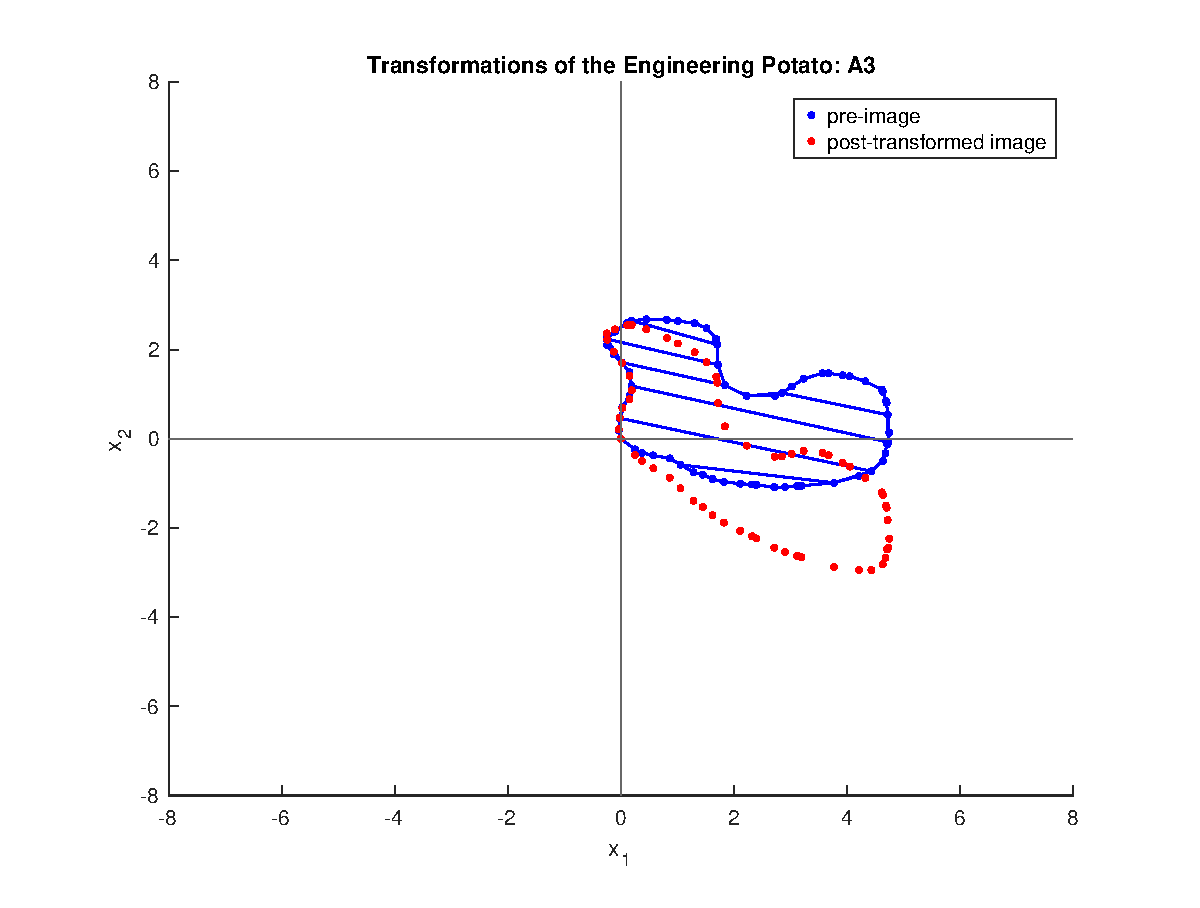
\includegraphics [width=4in]{4.eps}

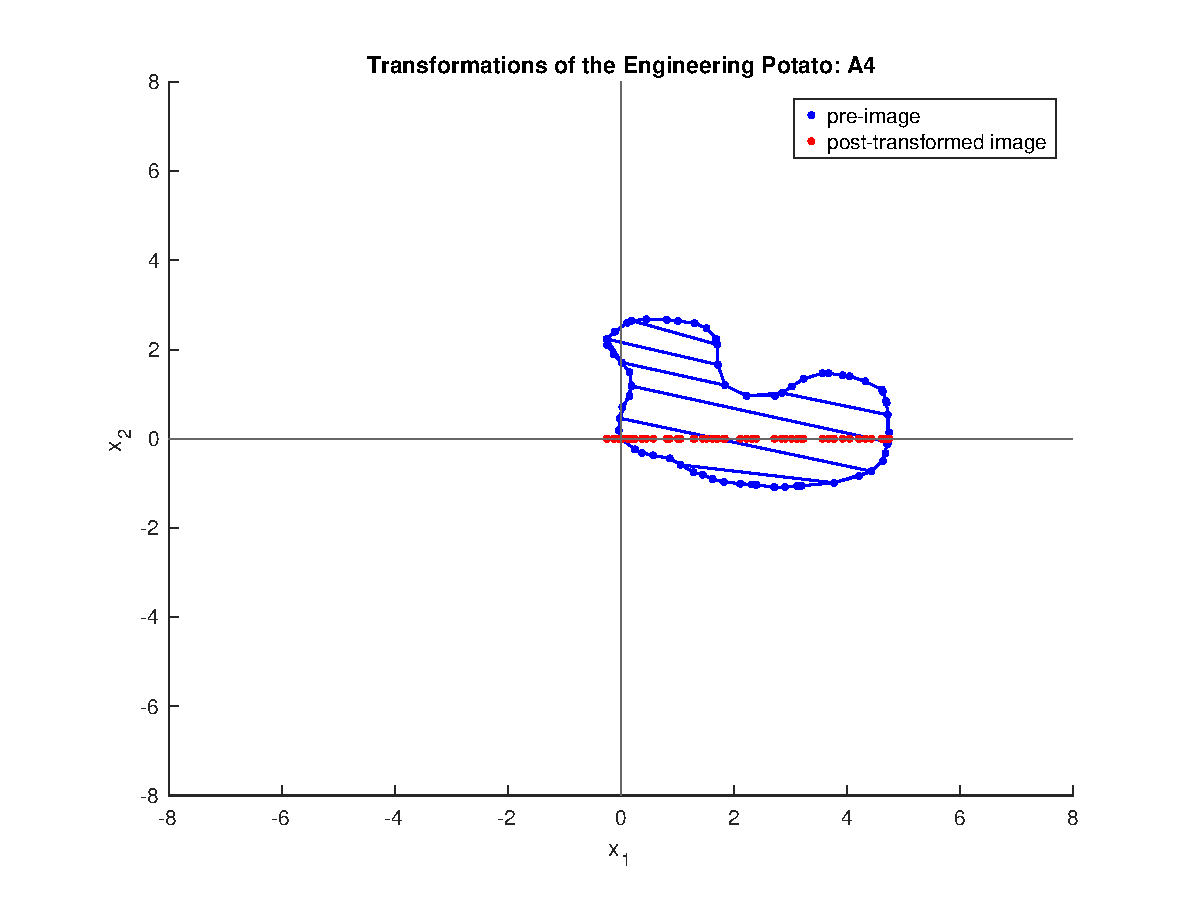
\includegraphics [width=4in]{5.eps}

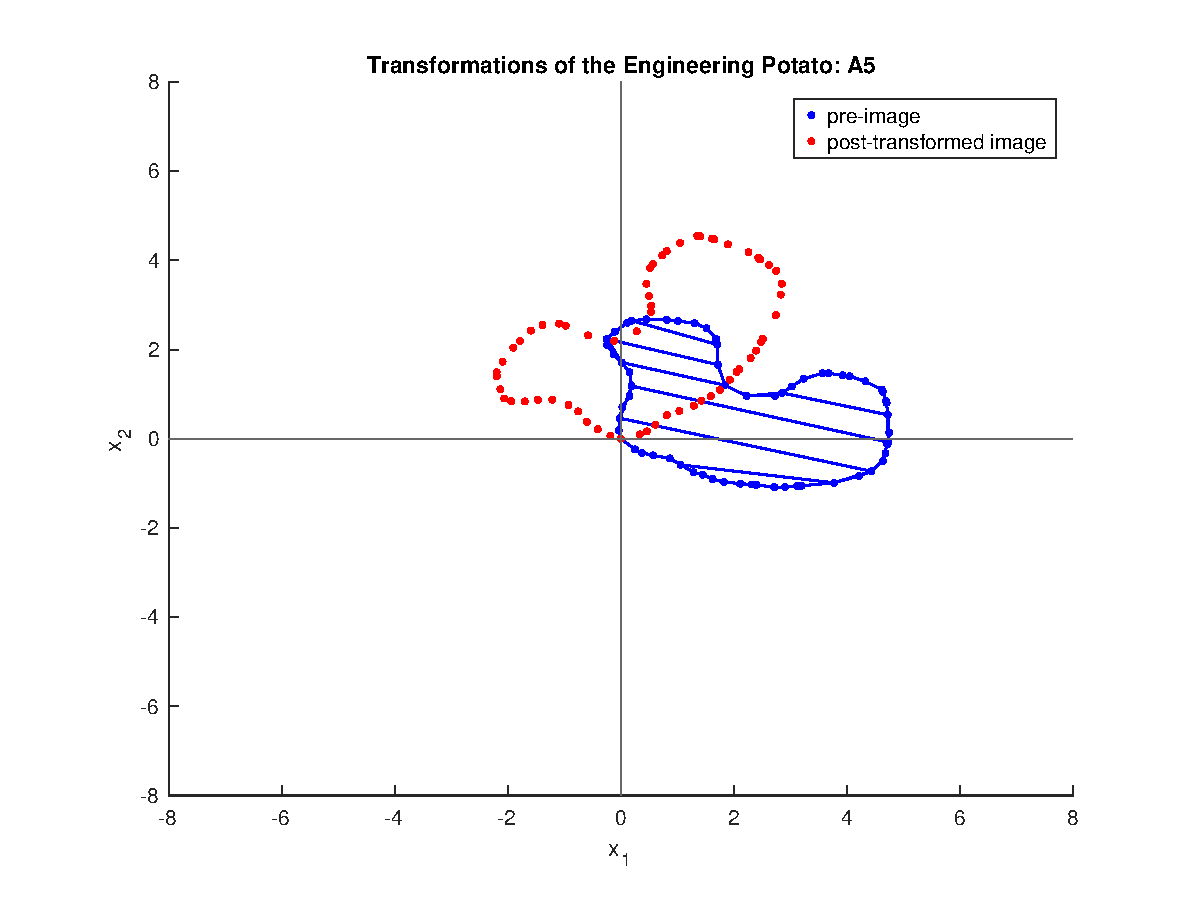
\includegraphics [width=4in]{6.eps}

\subsection*{E}

Since \(Area(C)= Area(B) \times |det(A)|\) then all transformations with \(-1 \leq det(A) \leq 1\) will preserve the area of the potato. Therefore, the transformations which preserve the area of the potato are \(\mathbf{I, III, V, (VI)}\).

\subsection*{F}

While \(|\det(A)| = 1\) guarantees that areas (or volumes) are preserved, it does not ensure that angles and distances between vectors are preserved. For instance, a tranformation could stretch the potato horizontally and shrink it vertically so that the area remains the same but the shape is now different.

\section*{2}

\subsection*{A}

\[
	\begin{aligned}
		\det(A) = & -1\bigl(5 \times 4 - 2 \times 3\bigr) - 1\bigl(5 \times 4 - 2 \times 2\bigr) + 2\bigl(5 \times 3 - 5 \times 2\bigr) \\
		=         & -1(20 - 6) - 1(20 - 4) + 2(15 - 10)                                                                                 \\
		=         & -14 - 16 + 10 = -20
	\end{aligned}
\]

\subsection*{B}

\[
	\begin{bmatrix}
		-1 & 1 & 2 \\
		5  & 5 & 2 \\
		2  & 3 & 4 \\
	\end{bmatrix}
	\xrightarrow{R_2 = R_2 + 5 R_1}
	\begin{bmatrix}
		-1 & 1  & 2  \\
		0  & 10 & 12 \\
		2  & 3  & 4  \\
	\end{bmatrix}
	\xrightarrow{R_3 = R_3 + 2 R_1}
	\begin{bmatrix}
		-1 & 1  & 2  \\
		0  & 10 & 12 \\
		0  & 5  & 8  \\
	\end{bmatrix}
	\xrightarrow{R_3 = R_3 - \frac{1}{2} R_2}
	\begin{bmatrix}
		-1 & 1  & 2  \\
		0  & 10 & 12 \\
		0  & 0  & 2  \\
	\end{bmatrix}
\]

\[
	det(A) = -1 \times 10 \times 2 = -20
\]

\subsection*{C}

\subsection*{I}

\[
	\\det(A) \;=\; (4)\times(-3)\times\bigl(0.5\bigr)\times(2)
\]
\[
	4 \times (-3) = -12
	\quad
	-12 \times 0.5 = -6
	\quad
	-6 \times 2 = -12
\]

\subsection*{II}

\[
	\det(B) = (4)\times(0)\times(0)\times(0) = 0.
\]

\subsection*{III}

\[
	\det(A^T A) \;=\; \det(A^T)\,\det(A)
\]
Moreover, $\det(A^T) = \det(A)$ for any square matrix $A$.
\[
	\det(A^T A) = \bigl(\det(A)\bigr)\,\bigl(\det(A)\bigr) = \bigl(\det(A)\bigr)^2
\]
\[
	\det(D) = \det(A^T A) = (-12)^2 = 144
\]

\subsection*{IV}

\[
	\det(A A^T) \;=\; \det(A)\,\det(A^T) \;=\; \bigl(\det(A)\bigr)^2
\]
\[
	\det(G) = (-12)^2 = 144.
\]



\section*{3}

\subsection*{A}

\subsubsection*{I}

\[
	\begin{aligned}
		p_1 = & \begin{bmatrix} 3 & -1 \\ -3 & 5\\ \end{bmatrix} \begin{bmatrix} -4 \\ -4 \\ \end{bmatrix} = \begin{bmatrix} 3 \times -4 + -1 \times -4 \\ -3 \times -4 + 5 \times -4 \\ \end{bmatrix} = \begin{bmatrix} -8 \\ -8 \\ \end{bmatrix}           \\
		p_2 = & \begin{bmatrix} 3 & -1 \\ -3 & 5\\ \end{bmatrix} \begin{bmatrix} -0.5 \\ 1.5 \\ \end{bmatrix} = \begin{bmatrix} 3 \times -0.5 + -1 \times 1.5 \\ -3 \times -0.5 + 5 \times 1.5 \\ \end{bmatrix} = \begin{bmatrix} -2.5 \\ 8 \\ \end{bmatrix} \\
		p_3 = & \begin{bmatrix} 3 & -1 \\ -3 & 5\\ \end{bmatrix} \begin{bmatrix} 4 \\ 1 \\ \end{bmatrix} = \begin{bmatrix} 3 \times 4 + -1 \times 1 \\ -3 \times 4 + 5 \times 1 \\ \end{bmatrix} = \begin{bmatrix} 11 \\ 2 \\ \end{bmatrix}                  \\
	\end{aligned}
\]


\begin{figure}[h!]
	\centering
	\begin{minipage}[b]{0.45\linewidth}
		\centering
		\begin{tikzpicture}[>=stealth, scale=0.6] % Adjust this value to change the size
			% Draw coordinate axes
			\draw[->] (-5,0) -- (5,0) node[right] {$x_1$};
			\draw[->] (0,-5) -- (0,5) node[above] {$x_2$};

			% Macro for drawing a vector from the origin.
			% Usage: \drawvector{x}{y}{Label}
			\newcommand{\drawvector}[3]{
				\draw[->, thick] (0,0) -- (#1,#2) node[above right] {$#3 = $ $\begin{pmatrix}#1\\#2\end{pmatrix}$ };
			}

			% Example vectors (replace/add your own vectors below)
			\drawvector{-1}{3}{v_1};
			\drawvector{1}{1}{v_2};
			\drawvector{-4}{-4}{r_1};
			\drawvector{-8}{-8}{p_1};

			% Optionally, mark the origin
			\fill (0,0) circle (2pt);
		\end{tikzpicture}
		\caption{\(r_1 \, , \, p_1\) pair}
	\end{minipage}
	\hfill
	\begin{minipage}[b]{0.45\linewidth}
		\centering
		\begin{tikzpicture}[>=stealth, scale=0.6]
			% Draw coordinate axes
			\draw[->] (-5,0) -- (5,0) node[right] {$x_1$};
			\draw[->] (0,-5) -- (0,5) node[above] {$x_2$};

			% Macro for drawing a vector from the origin.
			% Usage: \drawvector{x}{y}{Label}
			\newcommand{\drawvector}[3]{
				\draw[->, thick] (0,0) -- (#1,#2) node[above right] {$#3 = $ $\begin{pmatrix}#1\\#2\end{pmatrix}$ };
			}

			% Example vectors (replace/add your own vectors below)
			\drawvector{-1}{3}{v_1};
			\drawvector{1}{1}{v_2};
			\drawvector{-0.5}{1.5}{r_2};
			\drawvector{-2.5}{8}{p_2};

			% Optionally, mark the origin
			\fill (0,0) circle (2pt);
		\end{tikzpicture}
		\caption{\(r_2 \, , \, p_2\) pair}
	\end{minipage}
\end{figure}

\begin{figure}[h!]
	\centering
	\begin{tikzpicture}[>=stealth, scale=0.6]
		% Draw coordinate axes
		\draw[->] (-5,0) -- (5,0) node[right] {$x_1$};
		\draw[->] (0,-5) -- (0,5) node[above] {$x_2$};

		% Macro for drawing a vector from the origin.
		% Usage: \drawvector{x}{y}{Label}
		\newcommand{\drawvector}[3]{
			\draw[->, thick] (0,0) -- (#1,#2) node[above right] {$#3 = $ $\begin{pmatrix}#1\\#2\end{pmatrix}$ };
		}

		% Example vectors (replace/add your own vectors below)
		\drawvector{-1}{3}{v_1};
		\drawvector{1}{1}{v_2};
		\drawvector{4}{1}{r_3};
		\drawvector{11}{2}{p_3};

		% Optionally, mark the origin
		\fill (0,0) circle (2pt);
	\end{tikzpicture}
	\caption{\(r_3 \, , \, p_3 \) pair}
\end{figure}

\subsection*{B}

If the vector being transformed by \(A\) is a multiple of one of its eigenvectors, then the resulting vector remains in the direction of that eigenvector—it is simply scaled by the corresponding eigenvalue. This is because eigenvectors are, by definition, only scaled (not rotated) by the transformation. Therefore, any vector that is a multiple of an eigenvector is transformed into another multiple of that eigenvector.

\subsection*{C}
If
\[
	A\vec{v} = \lambda_v \vec{v}
\]
Then,
\[
	A(c\vec{v}) = c\,\lambda_v \vec{v}
\]
Therefore \(\vec{p}\) is an eigenvector of \(A\) with eigenvalue \(\lambda_p = \lambda_v \cdot c \).

\subsection*{D}

If a vector $\vec{v}$ is an eigenvector of a matrix \(A\), then I also know that any multiple of \(\vec{v}\). So there are infinitely many eigenvectors associated with that \(\lambda\)

\subsection*{E}

\textbf{Contents}

\begin{itemize}
	\setlength{\itemsep}{-1ex}
	\item YOUR CODE HERE
\end{itemize}
\begin{verbatim}
% Computational Linear Algebra (EK 103), Spring 2025, Boston University
% Problem Set 7, Question 3(d) code to help with finding eigenvalues/vectors
% March 2025

% Set up the workspace
clear all; close all; clc;
\end{verbatim}


\textbf{YOUR CODE HERE}

\begin{verbatim}
A = [3,-1;-3,5]

[V, D] = eig(A);
V
diag(D)
\end{verbatim}

\color{lightgray} \begin{verbatim}
A =

     3    -1
    -3     5


V =

   -0.7071    0.3162
   -0.7071   -0.9487


ans =

     2
     6

\end{verbatim} \color{black}

\section{4}

\subsection*{A}

\[
	A_2 - \lambda I =
	\begin{bmatrix}
		2 - \lambda & 14           \\
		0           & -5 - \lambda
	\end{bmatrix}
\]
Given \(det(A_2) = 0\)
\[
	(2 - \lambda)(-5 - \lambda) - 14 \times 0 = 0
\]
Therefore,
\[
	\lambda_1 = 2 \, , \, \lambda_2 -5
\]

\subsection*{B}

We need to prove that
\[
	(A- \lambda I) \vec{v} = 0
\]
has nontrivial solution. For \(\lambda_1 = 6\) we get

\[
	A- 6I=
	\begin{bmatrix}
		-3 & -1 \\
		-3 & -1
	\end{bmatrix}
\]

Then using row reduction we get

\[
	\xrightarrow{R_2 = R_2 - R_1}
	\begin{bmatrix}
		-3 & -1 \\
		0  & 0
	\end{bmatrix}
\]

Which has a free variable in the second column, and therefore has a nontrivial solution. For \(\lambda_2 = 2\) we get

\[
	A- 2I=
	\begin{bmatrix}
		1  & -1 \\
		-3 & 3
	\end{bmatrix}
\]

Then using row reduction we get

\[
	\xrightarrow{R_2 = R_2 + 3R_1}
	\begin{bmatrix}
		1 & -1 \\
		0 & 0
	\end{bmatrix}
\]

Which also has a free variable in the second column, and therefore has a nontrivial solution.

\subsection*{C}

For \(\lambda_1 = 2\)

\[
	A - 2I =
	\begin{bmatrix}
		0 & 14 \\
		0 & -7
	\end{bmatrix}
	\xrightarrow{R_2 = R_2 + \frac{1}{2}R_1}
	\begin{bmatrix}
		0 & 14 \\
		0 & 0
	\end{bmatrix}
\]

For \(\lambda_2 = -5\)

\[
	A + 5I =
	\begin{bmatrix}
		7 & 14 \\
		0 & 0
	\end{bmatrix}
\]

Which both prove the same point by previous logic.

\subsection*{D}

Solving for \(B\vec{x}=0\) where \(B = A_1 - \lambda_n I\)\\

For \(\lambda_1 = 6\)

\[
	B \vec{v_1} =
	\begin{bmatrix}
		-3 & -1 \\
		-3 & -1
	\end{bmatrix}
	\begin{bmatrix}
		x_1 \\
		x_2
	\end{bmatrix}
	=
	\begin{bmatrix}
		0 \\0
	\end{bmatrix}
\]
\[
	\xrightarrow{R_2 = R_2 - R_1}
	\begin{bmatrix}
		-3 & -1 \\
		0  & 0
	\end{bmatrix}
	\xrightarrow{R_1 = -\frac{1}{3}R_1}
	\begin{bmatrix}
		1 & \frac{1}{3} \\
		0 & 0
	\end{bmatrix}
\]
\[
	\therefore \vec{x} = \begin{bmatrix}
		-\frac{1}{3} t_2 \\
		t_2
	\end{bmatrix}
	= t_2 \begin{bmatrix}
		-\frac{1}{3} \\
		1
	\end{bmatrix}
\]
so the eigenspace for \(\lambda_1 = 6\) is
\[
	\left\{ t \begin{bmatrix}
		-\frac{1}{3} \\
		1
	\end{bmatrix} : t \in \mathbb{R} \right\}
\]


For \(\lambda_2 = 2\)

\[
	B \vec{v_1} =
	\begin{bmatrix}
		1  & -1 \\
		-3 & 3
	\end{bmatrix}
	\begin{bmatrix}
		x_1 \\
		x_2
	\end{bmatrix}
	=
	\begin{bmatrix}
		0 \\0
	\end{bmatrix}
\]
\[
	\xrightarrow{R_2 = R_2 + 3R_1}
	\begin{bmatrix}
		1 & -1 \\
		0 & 0
	\end{bmatrix}
\]
\[
	\therefore \vec{x} = \begin{bmatrix}
		-t_2 \\
		t_2
	\end{bmatrix}
	= t_2 \begin{bmatrix}
		-1 \\
		1
	\end{bmatrix}
\]
so the eigenspace for \(\lambda_2 = 2\) is
\[
	\left\{ t \begin{bmatrix}
		-1 \\
		1
	\end{bmatrix} : t \in \mathbb{R} \right\}
\]

\subsection*{E}

For \(\lambda_1 = 2\)

\[
    A_2 \vec{v_1} =
    \begin{bmatrix}
        2  & 14 \\
        0 & -5
    \end{bmatrix}
    \begin{bmatrix}
        x_1 \\
        x_2
    \end{bmatrix}
    =
    \begin{bmatrix}
        0 \\0
    \end{bmatrix}
\]
\[
    \xrightarrow{R_2 = R_2 + 0R_1}
    \begin{bmatrix}
        2 & 14 \\
        0 & -5
    \end{bmatrix}
\]
\[
    \therefore \vec{x} = \begin{bmatrix}
        -7t_1 \\
        0
    \end{bmatrix}
    = t_1 \begin{bmatrix}
        -7 \\
        0
    \end{bmatrix}
\]
so the eigenspace for \(\lambda_1 = 2\) is
\[
    \left\{ t \begin{bmatrix}
        -7 \\
        0
    \end{bmatrix} : t \in \mathbb{R} \right\}
\]

For \(\lambda_2 = -5\)

\[
    A_2 \vec{v_2} =
    \begin{bmatrix}
        7  & 14 \\
        0 & 0
    \end{bmatrix}
    \begin{bmatrix}
        x_1 \\
        x_2
    \end{bmatrix}
    =
    \begin{bmatrix}
        0 \\0
    \end{bmatrix}
\]
\[
    \xrightarrow{R_1 = \frac{1}{7}R_1}
    \begin{bmatrix}
        1 & 2 \\
        0 & 0
    \end{bmatrix}
\]
\[
    \therefore \vec{x} = \begin{bmatrix}
        -2t_2 \\
        t_2
    \end{bmatrix}
    = t_2 \begin{bmatrix}
        -2 \\
        1
    \end{bmatrix}
\]
so the eigenspace for \(\lambda_2 = -5\) is
\[
    \left\{ t \begin{bmatrix}
        -2 \\
        1
    \end{bmatrix} : t \in \mathbb{R} \right\}
\]

\end{document}